% BEGIN LICENSE BLOCK
% Version: CMPL 1.1
%
% The contents of this file are subject to the Cisco-style Mozilla Public
% License Version 1.1 (the "License"); you may not use this file except
% in compliance with the License.  You may obtain a copy of the License
% at www.eclipse-clp.org/license.
%
% Software distributed under the License is distributed on an "AS IS"
% basis, WITHOUT WARRANTY OF ANY KIND, either express or implied.  See
% the License for the specific language governing rights and limitations
% under the License.
%
% The Original Code is  The ECLiPSe Constraint Logic Programming System.
% The Initial Developer of the Original Code is  Cisco Systems, Inc.
% Portions created by the Initial Developer are
% Copyright (C) 2006 Cisco Systems, Inc.  All Rights Reserved.
%
% Contributor(s):
%
% END LICENSE BLOCK
%
% $Id: exthsusp.tex,v 1.7 2013/06/03 16:40:44 jschimpf Exp $
%

\chapter{Advanced Control Features}
%HEVEA\cutdef[1]{section}
\label{suspensions}

%-------
\section{Introduction}
%-------
This chapter introduces the control facilities that distinguish the
{\eclipse} language from Prolog by providing a computation
rule that is more flexible than simple left-to-right goal selection.
The core feature is the ability to suspend the execution of a goal
at some point during execution, and resume it under certain conditions
at a later stage.
Together with attributed variables, these facilities are the
prerequisites for the implementation of constraint propagation
and similar data-driven algorithms.

% Concepts
%       resolvent
%       execution model
%       floundering
% Delaying built-in predicates
% Support
% Declarative delay clauses
% The suspend predicate
% waking conditions (inst/bound/constrained, libraries, user-defined, symbolic,
% postponed)
% Lower-level primitives
%       The suspension
%       making suspensions
%       attaching suspensions to variables
%       attaching suspensions to triggers
% Demons
% More about Priorities
% details of waking, cut
% simulating alternative suspension facilities
%

%-------
\section{Concepts}
\subsection{The Structured Resolvent}
%-------
\index{resolvent}
The term \defnotion{resolvent} originates from Logic Programming.
It is the set of all goals that must be satisfied.
The computation typically starts with a resolvent consisting only of the
top-level goal
(the initial query).
This then gets successively transformed (by substituting goals that
match a clause head with an instance of the clause body, i.e., a
sequence of sub-goals),
and eventually terminates with one of the trivial goals
\notation{true} or \notation{fail}.
For example, given the program
\begin{quote}
\begin{verbatim}
p :- q, r.    % clause 1
q :- true.    % clause 2
r :- q.       % clause 3
\end{verbatim}
\end{quote}
and the goal p, the resolvent goes through the following states
before the goal is proven (by reduction to true) and the computation terminates:
\begin{quote}
\begin{verbatim}
p --1--> (q,r) --2--> (true,r) ----> (r) --3--> (q) --2--> true
\end{verbatim}
\end{quote}

\index{Prolog}
While in Prolog the resolvent is always processed from left to right
like in this example,
the resolvent in {\eclipse} is more structured, and can be manipulated
in a much more flexible way.
This is achieved by two basic mechanisms, \emph{suspension}
and \emph{priorities}.

\index{suspended goal}
Suspended goals form the part of the resolvent which is
currently not being considered. This is typically done when we
know that we cannot currently infer any interesting information from them.

\index{priority}
The remaining goals are ordered according to their priority.
At any time, the system attempts to solve the most urgent subgoal first.
{\eclipse} currently supports a fixed range of 12 different priorities,
priority 1 being the most urgent and 12 the least urgent.

Figure \ref{figresolv} shows the structure of the resolvent.
When a toplevel goal is launched, it has priority 12 and is the only
member of the resolvent. As execution proceeds, active goals may be
suspended, and suspended goals may be woken and scheduled with a
particular priority.
\begin{figure}
% picture has been made with xfig and exported as encapsulated postscript
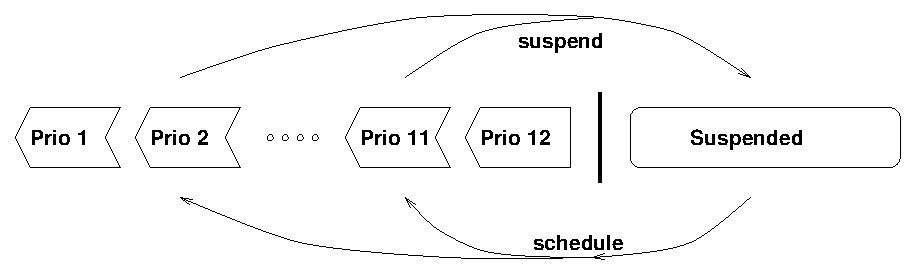
\includegraphics{resolv.eps}
\caption{Structure of the resolvent}
\label{figresolv}
\end{figure}

\subsection{Floundering}
\index{floundering}
The case that a subgoal remains suspended (delayed) at the end of the
computation
\index{floundering} is sometimes referred to as \defnotion{floundering}.
When floundering occurs, it means that the resolvent could not be reduced
to true or fail, and that the answer bindings that have been found
are valid only under the assumption that the remaining delayed goals
are in fact true. Since such a conditional answer is normally not
satisfactory (even though it may be correct), it is then necessary to change
the control aspect of the program.  The solution would usually be to either
make further variable instantiations or to change control annotations.
The aim is to get the delayed goals out of the suspended state and
into the scheduled state, where they will eventually be executed and reduced.
As a rule of thumb, goals will not suspend when all their arguments are
fully instantiated. Therefore, a program that makes sure that all its
variables are instantiated at the end of computation will typically not
suffer from floundering.


%----------------------------------------------------------------------
\section{Suspending Built-Ins and the Suspend-Library}
%----------------------------------------------------------------------

Basic {\eclipse} has two built-in predicates whose behaviour includes
suspending: the sound negation built-in
\txtbipref{\tld/1}{(~)/1}{../bips/kernel/control/T-1.html} and the sound disequality
predicate \txtbipref{\tld=/2}{(~=)/2}{../bips/kernel/termcomp/TE-2.html}.
Instead of succeeding or failing, they will suspend when their arguments
are insufficiently instantiated to make a decision. For example
\begin{quote}
\begin{verbatim}
?- X ~= 3.
X = X
There is 1 delayed goal.
Yes (0.00s cpu)
\end{verbatim}
\end{quote}
Here, the system does not have enough information to decide whether the
query is true or false. The goal remains delayed and we have a case of
floundering
(the {\eclipse} toplevel indicates this situation by printing a message
about delayed goals at the end of the computation).

However, when the variable which was responsible for the suspension gets
instantiated
later, the delayed goal will be resumed (woken) and either succeed, fail, or
suspend again. In the following example, the disequality predicate initially
suspends, but wakes up later and succeeds or fails, respectively:
\begin{quote}
\begin{verbatim}
?- X ~= 3, X = 4.
X = 4
Yes (0.00s cpu)
?- X ~= 3, X = 3.
No (0.00s cpu)
\end{verbatim}
\end{quote}


\label{suspendsolver}
Further predicate implementations with the same behaviour (delay until
all arguments are ground) can be found in the \libspec{suspend} library
\bipref{lib(suspend)}{../bips/lib/suspend/index.html}.
In particular, it implements all common arithmetic predicates plus
the constraints defined by the Common Arithmetic Solver Interface
(see Constraint Library Manual), for instance
\begin{verbatim}
=:=/2, =\=/2,  >=/2,  =</2,  >/2,  </2,
 $=/2, $\=/2, $>=/2, $=</2, $>/2, $</2,
 #=/2, #\=/2, #>=/2, #=</2, #>/2, #</2,
integers/1, reals/1
\end{verbatim}
The solver will suspend these predicates until all their arguments
are ground.\footnote{
Note that more powerful versions of these constraints exist in other
solvers such as the interval solver lib(ic).}

The suspend library is loaded into \eclipse\ on start-up, but the
constraints associated with the suspend solver are not imported.
To use them, either import the suspend library to the current module,
or call the constraint qualified with the module:
\begin{quote}
\begin{verbatim}
suspend:(X > 2), suspend:(X #=< 5)
\end{verbatim}
\end{quote}



%----------------------------------------------------------------------
\section{Development System Support}
%----------------------------------------------------------------------

As seen in the above example, the \index{top level loop} top level loop
indicates floundering by printing a message about delayed goals.
The command line toplevel then prompts and offers to print a list of
all delayed goals.
The Tkeclipse development environment provides better support in the form
of the Delayed Goals Viewer, which can be used to look at all delayed goals
or a filtered subset of them.

The tracer supports advanced control features via
the box-model ports DELAY and RESUME.
It also shows goal priorities (if they deviate from the default priority)
in angular brackets.


%----------------------------------------------------------------------
\section{Declarative Suspension: Delay Clauses}
%----------------------------------------------------------------------

For delaying calls to user-defined Prolog predicates, {\eclipse}
 provides several alternatives, the first being \defnotion{delay clauses}.
Delay clauses are a declarative means (they are in fact meta-clauses)
to specify the conditions under which the predicate should delay.
The semantics of delay clauses is thus cleaner than many alternative
approaches to delay primitives.

A delay clause is very similar to a normal Prolog clause. It has the form
\begin{quote}
\begin{verbatim}
delay <Head> if <Body>.
\end{verbatim}
\end{quote}
A predicate may have one or more delay clauses.
They have to be textually \emph{before} and \emph{consecutive}
with the normal clauses of the predicate they belong to.
The simplest example for a delay clause is one that checks if a variable
is instantiated:
\begin{quote}
\begin{verbatim}
delay report_binding(X) if var(X).
report_binding(X) :-
        printf("Variable has been bound to %w\n", [X]).
\end{verbatim}
\end{quote}

%----------------------------------------------------------------------
The operational semantics of the delay clauses is as follows:
when a procedure with delay clauses is called, then the delay
clauses are executed before executing the procedure itself.
If one of the delay clauses succeeds, the call is suspended,
otherwise they are all tried in sequence and,
if all delay clauses fail, the procedure is executed as usual.

The mechanism of executing a delay clause is similar to normal Prolog
clauses with two exceptions:
\begin{itemize}
\item the unification of the goal with the delay clause head is not the usual
Prolog unification, but rather unidirectional pattern matching
(see also section \ref{matching}).
\index{pattern matching}
\index{matching}
This means that the variables in the call cannot be bound
by the matching, if such a binding would be necessary to
perform the unification, it will fail instead.
For example, the head of the delay clause
\begin{quote}
\begin{verbatim}
delay p(a, X) if var(X).
\end{verbatim}
\end{quote}
does not match the goal \notation{p(A,~b)} but it matches the goal
\notation{p(a,~b)}.

\item the delay clauses are deterministic, they leave no choice points.
If one delay clause succeeds, the call is delayed and the following delay
clauses are not executed.
As soon as the call is resumed, all delay clauses that may succeed
are re-executed.
\end{itemize}
The reason for using pattern matching instead of unification
is to avoid a possible mixing of meta-level control with the
object level, similarly to \cite{dincbas84}.


%----------------------------------------------------------------------
The form of the head of a delay clause is not restricted.
For the body, the following conditions hold:

\begin{itemize}
\item the body subgoals must not bind any variable in the call and they
must not delay themselves.
The system does not verify these conditions currently.

\item it should contain at least one of the following subgoals:
\begin{itemize}
\item \bipref{var/1}{../bips/kernel/typetest/var-1.html}
\item \bipref{nonground/1}{../bips/kernel/typetest/nonground-1.html}
\item \predspec{nonground/2} (see
  \bipref{nonground/3}{../bips/kernel/typetest/nonground-3.html})
\item \predspec{\bsl==/2}
\index{\bsl==/2@\bsl\notation{==/2}}
\end{itemize}
If this is not the case, then the predicate may delay without being linked
to a variable, so it delays forever and cannot be woken again.
Experience shows that the above four primitives suffice to express most
usual conditions.
\end{itemize}

\subsubsection{More Examples}
\begin{itemize}
\item
A predicate that checks if its argument is a proper list of integers.
The delay conditions specify that the predicate should delay if the list
is not terminated or if it contains variable elements.
This makes sure that it will never generate list elements, but only
acts as a test:
\begin{quote}
\begin{verbatim}
delay integer_list(L) if var(L).
delay integer_list([X|_]) if var(X).
integer_list([]).
integer_list([X|T]) :- integer(X), integer_list(T).
\end{verbatim}
\end{quote}

\item
Delay if the first two arguments are identical and the third is a variable:
\begin{quote}
\begin{verbatim}
delay p(X, X, Y) if var(Y).
\end{verbatim}
\end{quote}

\item
Delay if the argument is a structure whose first subterm is not ground:
\begin{quote}
\begin{verbatim}
delay p(X) if compound(X), arg(1, X, Y), nonground(Y).
\end{verbatim}
\end{quote}

\item
Delay if the argument term contains 2 or more variables:
\begin{quote}
\begin{verbatim}
delay p(X) if nonground(2, X).
\end{verbatim}
\end{quote}

\item
The
\predspec{\bsl==/2}
\index{\bsl==/2@\bsl\notation{==/2}}
predicate as a delaying condition is useful mainly
in calls like \notation{X~+~Y~=~Z} which need not be delayed if
\about{X}~\notation{==}~\about{Z}.
\about{Y} can be directly bound to 0, provided that \about{X} is later bound to
a number
(or it is not bound at all)
The condition \notation{X {\bsl}== Y} makes sense
only if \about{X} or \about{Y} are nonground: a delay clause
\begin{quote}
\begin{verbatim}
delay p(X, Y) if X \== Y.
\end{verbatim}
\end{quote}
executed with the call \notation{?- p(a, b)} of course succeeds and the call
delays
forever, since no variable binding can wake it.
\end{itemize}

\textbf{CAUTION}: It may happen that the symbol \notation{:-} is erroneously
used instead of \notation{if} in the delay clause. To indicate this error,
the compiler complains about redefinition of the built-in predicate
\predspec{delay/1}.


%----------------------------------------------------------------------
\section{Explicit suspension with \predspec{suspend/3}}
%----------------------------------------------------------------------
\label{suspend3}
While delay-clauses are an elegant, declarative way of specifying how
a program should execute, it is sometimes necessary to be more explicit
about suspension and waking conditions.
The built-in predicate
\bipref{suspend/3}{../bips/kernel/suspensions/suspend-3.html}
is provided for this purpose\footnote{
\predspec{suspend/3} is itself based on the lower-level primitives
\predspec{make_suspension/3}
and \predspec{insert_suspension/4}, which are described below.}.
It allows one to explicitly create a suspended goal, specify its priority
and its exact waking conditions.

When
\begin{quote}
\predspec{suspend(\pattern{Goal}, \pattern{Prio}, \pattern{CondList})}
\end{quote}
is called, \about{Goal} will be suspended with priority \about{Prio}
and it will wake up
as soon as one of the conditions specified in the \about{CondList}
is satisfied.
This list contains specifications of the form
\begin{quote}
\notation{\pattern{Vars} \notation{->} \pattern{Cond}}
\end{quote}
to denote that as soon as one of the variables in the term \about{Vars}
satisfies the condition \about{Cond}, the suspended goal will
be woken and then executed as soon as the program priority allows it.
\about{CondList} can also be a single specification.

The condition \about{Cond} can be the name of a system-defined waking condition,
e.g.,
\begin{quote}
\begin{verbatim}
[X,Y]->inst
\end{verbatim}
\end{quote}
means that as soon as one (or both) of the variables \about{X}, \about{Y}
is instantiated, the suspended goal will be woken.
\index{suspending variables}
These variables are also called the \defnotion{suspending variables} of the
goal.


\about{Cond} can also be the specification of a suspension list
defined in one of currently loaded library attributes. For example, when the
interval solver library lib(ic) is loaded, either of
\begin{quote}
\begin{verbatim}
[A,B]->ic:min
[A,B]->ic:(min of ic)
\end{verbatim}
\end{quote}
triggers the suspended goal as soon as the minimum element
of the domain of either \about{A} or \about{B} are updated
(see Constraint Library Manual, IC Library).

Another admissible form of condition \about{Cond} is
\begin{quote}
\begin{verbatim}
trigger(Name)
\end{verbatim}
\end{quote}
which suspends the goal on the global trigger condition \about{Name}
(see section~\ref{trigger}).


Using
\bipref{suspend/3}{../bips/kernel/suspensions/suspend-3.html},
we can rewrite our first delay-clause example from above as follows:
\begin{quote}
\begin{verbatim}
report_binding(X) :-
        ( var(X) ->
            suspend(report_binding(X), 0, X->inst)
        ;
            printf("Variable has been bound to %w\n", [X])
        ).
\end{verbatim}
\end{quote}
Here, when the predicate is called with an uninstantiated argument,
we explicitly suspend a goal with the condition that it be woken as
soon as X becomes instantiated. The priority is given as 0, which indicates
the default priority (0 is not a valid priority itself).
Running this code produces the following:
\begin{quote}
\begin{verbatim}
?- report_binding(X).
X = X
There is 1 delayed goal.
Yes (0.00s cpu)
\end{verbatim}
\end{quote}
When X is later instantiated, it will wake up and print the message:
\begin{quote}
\begin{verbatim}
?- report_binding(X), writeln(here), X = 99.
here
Variable has been bound to 99
X = 99
Yes (0.00s cpu)
\end{verbatim}
\end{quote}



%----------------------------------------------------------------------
\section{Waking conditions}
%----------------------------------------------------------------------
The usual purpose of suspending a goal is to wait and resume it later
when more information about its arguments is available.
In Logic Programming, this is usually the case when certain events
related to variables occur.
When such an event occurs, the suspended goal is passed to the
waking scheduler which puts it at the appropriate place
in the priority queue of woken goals and as soon as it becomes
first in the queue, the suspended goal is executed.

The event which causes a suspended goal to be woken is usually
related to one or more variables, for example
variable instantiation, or a modification of a variable's
attribute.
However, it is also possible to trigger suspension with symbolic events
not related to any variable.


%----------------------------------------------------------------------
\subsection{Standard Waking Conditions on Variables}
%----------------------------------------------------------------------
\label{suspend}
\index{suspend}
\index{coroutining}
\label{coroutining}%
There are three very general standard waking conditions which
can be used with any variable. They are, in order of increasing generality:
\begin{quote}
\begin{description}
\item[inst:] wake when a variable gets instantiated;
\item[bound:] wake when a variable gets instantiated or bound to
        another variable;
\item[constrained:] wake when a variable gets instantiated or bound to
        another variable or becomes otherwise constrained.
\end{description}
\end{quote}
Each condition subsumes the preceding, more specific ones.


% - - - - - - - - - - - - - - - - - - - - - - - - - - - - - - - - - -
\subsubsection{Waking on Instantiation: inst}
% - - - - - - - - - - - - - - - - - - - - - - - - - - - - - - - - - -

To wake a goal when a variable gets instantiated, the \notation{inst}
condition is used. For example the following code suspends a goal until
variable \about{X} is instantiated:
\begin{quote}
\begin{verbatim}
?- suspend(writeln(woken(X)), 0, X->inst).
X = X
There is 1 delayed goal.
Yes (0.00s cpu)
\end{verbatim}
\end{quote}
If this variable is later instantiated (bound to a non-variable),
the goal executes in a data-driven way:
\begin{quote}
\begin{verbatim}
?- suspend(writeln(woken(X)), 0, X->inst), X = 99.
woken(99)
X = 99
Yes (0.00s cpu)
\end{verbatim}
\end{quote}
If we specify several instantiation conditions for the same goal,
the goal will wake up as soon as the first of them occurs:
\begin{quote}
\begin{verbatim}
?- suspend(writeln(woken(X,Y)), 0, [X,Y]->inst), X = 99.
woken(99, Y)
X = 99
Y = Y
Yes (0.00s cpu)
\end{verbatim}
\end{quote}
It is not possible to specify a conjunction of conditions directly!

Let us now suppose we want to implement a predicate \predspec{succ/2}, such that
\notation{succ(X,~Y)}
is true when \about{Y} is the next integer after \about{X}. If we want the
predicate
to act as a lazy test, we must let it suspend until both variables
are instantiated. This can be programmed as follows:
\begin{quote}
\begin{verbatim}
succ_lazy(X, Y) :-
        ( var(X) -> suspend(succ_lazy(X,Y), 0, X->inst)
        ; var(Y) -> suspend(succ_lazy(X,Y), 0, Y->inst)
        ; Y =:= X+1
        ).
\end{verbatim}
\end{quote}
The conjunctive condition ``wait until \about{X} and \about{Y} are
instantiated''
is
implemented by first waiting for \about{X}'s instantiation, then waking up and
re-suspending waiting for \about{Y}'s instantiation.

A more eager implementation of \predspec{succ/2} would delay only until
a single variable argument is left, and then compute the variable from
the nonvariable argument:
\begin{quote}
\begin{verbatim}
succ_eager(X, Y) :-
        ( var(X) ->
            ( var(Y) ->
                suspend(succ_eager(X,Y), 0, [X,Y]->inst)
            ;
                X is Y-1
            )
        ;
            Y is X+1
        ).
\end{verbatim}
\end{quote}
Here, we suspend only in the case that both arguments are variables,
and wake up as soon as either of them gets instantiated.

Waiting for groundness of a term can be done in a way similar to the
way \predspec{succ_lazy/2} waited for both arguments to be instantiated: we
pick
any variable in the nonground term and wait for its instantiation.
If this happens, we check whether other variables remain, and if yes,
we re-suspend on one of the remaining variables. The following predicate
waits for a term to become ground, and then calls arithmetic evaluation on it:
\begin{quote}
\begin{verbatim}
eval_lazy(Expr, Result) :-
        ( nonground(Expr, Var) ->
            suspend(eval_lazy(Expr,Result), 0, Var->inst)
        ;
            Result is Expr
        ).
\end{verbatim}
\end{quote}
We have used the built-in predicate
\bipref{nonground/2}{../bips/kernel/typetest/nonground-2.html}
which tests a term for groundness and returns one of its variables
if it is nonground. Note also that in this implementation the same
\predspec{eval_lazy/2} goal gets woken and re-suspended possibly many times.
See section \ref{secdemon} below for how to address this inefficiency.


% - - - - - - - - - - - - - - - - - - - - - - - - - - - - - - - - - -
\subsubsection{Waking on Binding: bound}
% - - - - - - - - - - - - - - - - - - - - - - - - - - - - - - - - - -

Sometimes it is interesting to wake a goal when the number of variables
among its arguments is reduced. This happens not only when a variable
disappears due to instantiation, but also when two variables get unified
(the result being a single variable). Consider the \predspec{succ_eager/2}
predicate
above: we know that a goal like \notation{succ_eager(X,X)}. must always fail
because an integer cannot be equal to its successor. However, the above
implementation does not detect this case until X gets instantiated.

The \notation{bound} waking condition subsumes the \notation{inst} condition,
but
also wakes when any two of the variables in the condition specification get
unified with each other (aliased).
Using this property, we can improve the implementation of
\predspec{succ_eager/2}
as follows:
\begin{quote}
\begin{verbatim}
succ_eager1(X, Y) :-
        ( var(X) ->
            ( var(Y) ->
                X \== Y,
                suspend(succ_eager1(X,Y), 0, [X,Y]->bound)
            ;
                X is Y-1
            )
        ;
            Y is X+1
        ).
\end{verbatim}
\end{quote}
This gives us the desirable behaviour of failing as soon as possible:
\begin{quote}
\begin{verbatim}
?- succ_eager1(X, Y), X = Y.
No (0.00s cpu)
\end{verbatim}
\end{quote}
Note that the built-in predicate
\txtbipref{\tld=/2}{(~=)/2}{../bips/kernel/termcomp/TE-2.html}
is a similar case and uses the \notation{bound} waking condition for the
same reason.



% - - - - - - - - - - - - - - - - - - - - - - - - - - - - - - - - - -
\subsubsection{Waking on Constraining: constrained}
% - - - - - - - - - - - - - - - - - - - - - - - - - - - - - - - - - -

In plain Prolog, variable instantiation is the only way in which a single
variable can become more constrained.  In the presence of constraints,
there are other ways. The most obvious example are variable domains:
when a variable's domain gets reduced, the variable becomes more
constrained. This means that a delayed goal that previously still had
a chance to succeed, could now have become impossible to satisfy,
and should therefore be checked again.

The purpose of the \notation{constrained} waking condition is to make it
possible to wake a suspended goal whenever a variable becomes more
constrained in a general sense. Having this general notion
of constrained-ness makes it possible to write generic libraries
that do interesting things with constraints and constrained variables
without their implementation having to be linked to a particular
constraint-solver\footnote{%
  Examples of such libraries are \libspec{branch_and_bound},
  \libspec{changeset}, \libspec{chr}/\libspec{ech}, \libspec{propia},
  \libspec{repair}, \libspec{visualisation}.}.

The \notation{constrained} waking condition subsumes the \notation{bound}
condition
(which in turn subsumes the \notation{inst} condition).
While goals suspended on the \notation{inst} and \notation{bound} conditions
are woken implicitly by the unification routine, libaries which implement
domain variables are responsible for notifying the system when they
constrain a variable. They do so by invoking the built-ins
\bipref{notify_constrained/1}{../bips/kernel/suspensions/notify_constrained-1.html}
and \bipref{wake/0}{../bips/kernel/suspensions/wake-0.html}
which is the generic way of telling the system that a variable has been
constrained.

The simplest application using the \notation{constrained} condition is a little
debugging support predicate that prints a variable's current partial value
(e.g., domain) whenever it changes:
\begin{quote}
\begin{verbatim}
report(X) :-
        ( var(X) ->
            writeln(constrained(X)),
            suspend(report(X), 1, X->constrained)  % (re)suspend
        ;
            writeln(instantiated(X))
        ).
\end{verbatim}
\end{quote}
This now works with any library that implements a notion of constrainedness,
e.g., the interval solver library(ic):
\begin{quote}
\begin{verbatim}
?- report(X), X :: 1..5, X #> 2, X #< 4.
constrained(X)
constrained(X{1 .. 5})
constrained(X{3 .. 5})
instantiated(3)
X = 3
Yes (0.01s cpu)
\end{verbatim}
\end{quote}
The \predspec{report/1} predicate is woken when the domain is initally attached
to X,
whenever the domain gets reduced, and finally when X gets instantiated.



%----------------------------------------------------------------------
\subsection{Library-defined Waking Conditions on Variables}
%----------------------------------------------------------------------

Constraint-solver libraries typically define additional, specialised
waking conditions for the type of variable that they implement.
For instance, the interval solver lib(ic) defines the following
conditions:
\begin{quote}
\begin{description}
\item[min:] wake when the minimum domain value changes;
\item[max:] wake when the maximum domain value changes;
\item[hole:] wake when the domain gets a new hole;
\item[type:] wake when the variable type changes from real to integer.
\end{description}
\end{quote}
Obviously, these conditions only make sense for domain variables
that are created by the lib(ic) library, and are mainly useful for
implementing extensions to this library, e.g., new constraints.
The library-defined waking conditions can be used with
\bipref{suspend/3}{../bips/kernel/suspensions/suspend-3.html}
by using one of the following syntactic forms:
\begin{quote}
\begin{verbatim}
[A, B]->ic:min
[A, B]->ic:(min of ic)
\end{verbatim}
\end{quote}
Using these conditions, we can define a more specialised form of
the above \predspec{report/1} predicate which only wakes up on the specified
ic-domain changes:
\begin{quote}
\begin{verbatim}
report_ic(X) :-
        ( var(X) ->
            writeln(newdomain(X)),
            suspend(report_ic(X), 1, [X->ic:min,X->ic:max,X->ic:hole])
        ;
            writeln(instantiated(X))
        ).
\end{verbatim}
\end{quote}
The behaviour is similar to above, the predicate wakes up on every
domain change:
\begin{quote}
\begin{verbatim}
?- X::1..5, report_ic(X), X#> 2, X #< 4.
newdomain(X{1 .. 5})
newdomain(X{3 .. 5})
instantiated(3)
X = 3
Yes (0.00s cpu)
\end{verbatim}
\end{quote}
Note that we now have to set up the delayed goal \emph{after} the
variable already has a domain. This is because the ic-specific waking
conditions can only be used with ic-variables,\footnote{%
  More precisely,
  variables which have an ic-attribute, see chapter \ref{attrvars}.}
not with domain-less generic variables.



%----------------------------------------------------------------------
\subsection{Global Symbolic Waking Conditions: Triggers}
\label{trigger}
%----------------------------------------------------------------------

Although waking conditions for a goal are usually related to variables
within the goal's arguments, it is also possible to specify symbolic
waking conditions which are unrelated to variables.
\index{trigger}\index{symbolic waking condition}%
These are called \defnotion{triggers} and are identified simply by an
arbitrary name (an atom). Goals can be suspended on such triggers,
and the trigger can be pulled explicitly by program code in
particular circumstances. By combining triggers with the event mechanism
\index{events}
(chapter \ref{chapexcept}) it is even possible to wake goals in
response to synchronous or asynchronous events.

A goal is suspended on a trigger using the syntax \pattern{trigger(Name)}
in \bipref{suspend/3}{../bips/kernel/suspensions/suspend-3.html}
as in the following example:
\begin{quote}
\begin{verbatim}
?- suspend(writeln(woken), 0, trigger(happy)).
There is 1 delayed goal.
Yes (0.00s cpu)
\end{verbatim}
\end{quote}
The built-in
\bipref{trigger/1}{../bips/kernel/suspensions/trigger-1.html}
can then be used to wake the goal:
\begin{quote}
\begin{verbatim}
?- suspend(writeln(woken), 0, trigger(happy)), trigger(happy).
woken
Yes (0.00s cpu)
\end{verbatim}
\end{quote}
Of course, symbolic triggers can be used together with other
waking conditions to specify alternative reasons to wake a goal.



% - - - - - - - - - - - - - - - - - - - - - - - - - - - - - - - - - -
\subsubsection{Postponed Goals}
% - - - - - - - - - - - - - - - - - - - - - - - - - - - - - - - - - -
\index{postponed}
There is one system-defined trigger called \defnotion{postponed}.%
\index{postponed trigger}\index{trigger!postponed}
It is provided as a way to postpone the triggering of a goal as much
as possible. This trigger is pulled just before the end of
certain encapsulated executions, like
\begin{itemize}
\item end of toplevel execution;
\item inside all-solution predicates
  (\bipref{findall/3}{../bips/kernel/allsols/findall-3.html},
  \bipref{setof/3}{../bips/kernel/allsols/setof-3.html});
\item inside \bipref{bb_min/3}{../bips/lib/branch_and_bound/bb_min-3.html} and
  \bipref{minimize/2}{../bips/lib/branch_and_bound/minimize-2.html}.
\end{itemize}
A suspension should be attached to the \notation{postponed} trigger only when
\begin{itemize}
\item it might not have any other waking conditions left;
\item and it might at the same time have other waking conditions left
        that could make it fail during further execution;
\item and one does not want to execute it now, e.g., because it is known
        to succeed or re-suspend.
\end{itemize}
An example is a goal that originally woke on modifications of the upper
bound of an interval variable. If the variable gets instantiated to its
upper bound, there is no need to wake the goal (since the bound has not
changed), but the variable (and with it the waking condition) disappears
and the goal may be left orphaned.




%----------------------------------------------------------------------
\section{Lower-level Primitives}
%----------------------------------------------------------------------

Suspended goals are actually represented by a special
opaque data type, called \defnotion{suspension}, which can be explicitly
manipulated under program control using the primitives defined in
this section.
Although usually a suspended goal waits for some waking condition
in order to be reactivated, the primitives for suspension handling
do not enforce this. To provide maximum flexibility of use,
the functionalities of suspending and waking/scheduling are
separated from the trigger mechanisms that cause the waking.


\index{suspension|(}

\subsection{Suspensions and Suspension Lists}
%-------
A suspension represents a goal that is part of the resolvent.
Apart from the goal structure proper, it holds information that
is used for controlling its execution.
The components of a suspension are:
\begin{quote}
\begin{description}
\item[The goal structure]
        A term representing the goal itself, e.g., \notation{X > Y}.
\item[The goal module]
        The module from which the goal was called.
\item[The scheduling priority]
        The priority with which the goal will be scheduled when
        it becomes woken.
\item[The run priority]
        The priority under which the goal will eventually be executed.
\item[The state]
        This indicates the current position of the suspension within
        the resolvent. It is either suspended (sleeping), scheduled
	or executed (dead).
\item[Additional data]
	Debugging information etc.
\end{description}
\end{quote}

Suspensions which should be woken by the same event are grouped
together in a \defnotion{suspension list}.
%This is a normal Prolog list which contains suspensions.
Suspension lists are either stored in an attribute of
an attributed variable or attached to a symbolic trigger.


\subsection{Creating Suspended Goals}
%-------
\index{suspension!creating}
The most basic primitive to create a suspension is
\begin{quote}
\biptxtrefni{make_suspension(\pattern{Goal},~\pattern{Priority},%
~\pattern{Susp} \lbr, \pattern{Module}\rbr)}{make_suspension/3,4}{../bips/kernel/suspensions/make_suspension-3.html}%
\indextt{make_suspension/3}\indextt{make_suspension/4}
\end{quote}
where \about{Goal} is the goal structure,
\about{Priority} is a small integer denoting the priority with which
the goal should be woken and \about{Susp} is the resulting suspension.

Note that usually
\biprefni{make_suspension/3,4}{../bips/kernel/suspensions/make_suspension-3.html}
is not used directly, but implicitly via
\biprefni{suspend/3,4}{../bips/kernel/suspensions/suspend-3.html}\indextt{suspend/3}\indextt{suspend/4}
(described in section \ref{suspend3}) which in addition attaches the suspension
to a
trigger condition.

A suspension which has not yet been scheduled
for execution and executed, is called
\defnotionni{sleeping},\index{sleeping suspension}\index{suspension!sleeping}
a suspension which has already been executed is called
\defnotionni{executed}\index{executed suspension}\index{suspension!executed}
or
\defnotionni{dead}\index{dead suspension}\index{suspension!dead}
(since it disappears from the resolvent,
but see section \ref{secdemon} for an exception).
A newly created suspension is always sleeping, however
note that due to backtracking, an executed suspension
can become sleeping again.
Sometimes we use the term
\defnotion{waking},\index{waking suspension}\index{suspension!waking}
which is less precise and
denotes the process of both scheduling and eventual execution.


By default, suspensions are printed as follows (the variants with invocation
numbers are used when the debugger is active):
\begin{center}
\begin{tabular}{|c|l|}
\hline
'SUSP-_78-susp'		&   sleeping suspension with id _78 \\
'SUSP-_78-sched'	&   scheduled suspension with id _78 \\
'SUSP-_78-dead'		&   dead suspension with id _78 \\
\hline
'SUSP-123-susp'		&   sleeping suspension with invocation number 123 \\
'SUSP-123-sched'	&   scheduled suspension with invocation number 123 \\
'SUSP-123-dead'		&   dead suspension with id invocation number 123 \\
\hline
\end{tabular}
\end{center}
It is possible to change the way suspensions are printed by defining a
\bipref{portray/3}{../bips/kernel/syntax/portray-3.html}
transformation for the term type \notation{goal}.



\subsection{Operations on Suspensions}
%-------
The following summarises the predicates that can be used to create, test,
decompose and destroy suspensions.
\begin{quote}
\begin{description}
\item[\biptxtref{make_suspension(\pattern{Goal},~\pattern{Priority},~\pattern{Susp})}{make_suspension/3}{../bips/kernel/suspensions/make_suspension-3.html}]
\item[\biptxtref{make_suspension(\pattern{Goal},~\pattern{Priority},~\pattern{Susp},~\pattern{Module})}{make_suspension/4}{../bips/kernel/suspensions/make_suspension-4.html}]
Create a suspension with a given priority from a given goal.
The goal will subsequently show up as a delayed goal.

\item[\biptxtref{is_suspension(\pattern{Susp})}{is_suspension/1}{../bips/kernel/typetest/is_suspension-1.html}]
Succeeds if \about{Susp} is a sleeping or scheduled suspension,
fails if it is not a suspension or a suspension that has been already executed.

\item[\biptxtref{type_of(\pattern{S},~\pattern{goal})}{type_of/2}{../bips/kernel/typetest/type_of-2.html}]
Succeeds if \about{S} is a suspension, no matter if it is
sleeping, scheduled or executed.

\item[\biptxtref{get_suspension_data(%
\pattern{Susp},~\pattern{Name},~\pattern{Value})}{get_suspension_data/3}{../bips/kernel/suspensions/get_suspension_data-3.html}]
Extract any of the information contained in the suspension:
\about{Name} can be one of
\notation{goal}, \notation{module}, \notation{priority}, \notation{state} or
\notation{invoc} (debugger invocation number).


\item[\biptxtref{set_suspension_data(%
\pattern{Susp},~\pattern{Name},~\pattern{Value})}{set_suspension_data/3}{../bips/kernel/suspensions/set_suspension_data-3.html}]
The \notation{priority} and \notation{invoc} (debugger invocation number) fields
of a suspension can be changed using this primitive.
If the priority of a sleeping suspension is changed,
this will only have an effect at the time the suspension gets
scheduled. If the suspension is already scheduled, changing
priority has no effect, except for future schedulings of demons
(see~\ref{secdemon}).


\item[\biptxtref{kill_suspension(\pattern{Susp})}{kill_suspension/1}{../bips/kernel/suspensions/kill_suspension-1.html}]
Convert the suspension \about{Susp} into an executed
one, i.e., remove the suspended goal from the resolvent.
This predicate is meta-logical as its use may
change the semantics of the program.
\end{description}
\end{quote}



\subsection{Examining the Resolvent}
%-------
The system keeps track of all created suspensions and it
uses this data, e.g., in the built-in predicates
\bipref{delayed_goals/1}{../bips/kernel/suspensions/delayed_goals-1.html},
\bipref{suspensions/1}{../bips/kernel/suspensions/suspensions-1.html},
\bipref{current_suspension/1}{../bips/kernel/suspensions/current_suspension-1.html},
\bipref{subcall/2}{../bips/kernel/suspensions/subcall-2.html}
\index{floundering}
and to detect floundering of the query given to the {\eclipse} top-level loop.



\subsection{Attaching Suspensions to Variables}
%---------


Suspensions are attached to variables by means of the attribute mechanism.
\index{attribute}
For this purpose, a variable attribute must have one or more slots
reserved for \defnotionni{suspension lists}.\index{suspension list}
Suspensions can then be inserted into one or several of those lists using
\begin{quote}
\begin{description}
\item[\biptxtref{insert_suspension(\pattern{Vars},~\pattern{Susp},~\pattern{Index})}{insert_suspension/3}{../bips/kernel/suspensions/insert_suspension-3.html}]
Insert the suspension \about{Susp} into the \about{Index}'th
suspension list of all attributed variables occurring in \about{Vars}.
The current module specifies which of the attributes will be taken.

\item[\biptxtref{insert_suspension(\pattern{Vars},~\pattern{Susp},~\pattern{Index},~\pattern{Module})}{insert_suspension/4}{../bips/kernel/suspensions/insert_suspension-4.html}]
Similar to the above,
but it inserts the suspension into the attribute specified by \about{Module}.
\end{description}
\end{quote}

For instance,
\begin{quote}
\begin{verbatim}
insert_suspension(Vars, Susp, inst of suspend, suspend)
\end{verbatim}
\end{quote}
inserts the suspension into the \notation{inst}
list of the (system-predefined) \notation{suspend}
attribute of all variables that occur in \about{Vars}, and
\begin{quote}
\begin{verbatim}
insert_suspension(Vars, Susp, max of fd, fd)
\end{verbatim}
\end{quote}
would insert the suspension into the \notation{max} list of the finite-domain
attribute of all variables in \about{Vars}.

Note that both predicates
find all attributed variables which occur in the general term \about{Vars} and
for
each of them,
locate the attribute which corresponds to the current module or the
\about{Module} argument respectively.
This attribute must be a structure, otherwise an error
is raised, which means that the attribute has to be initialized
before calling
\biprefni{insert_suspension/4,3}{../bips/kernel/suspensions/insert_suspension-4.html}.%
\indextt{insert_suspension/3}\indextt{insert_suspension/4}
Finally, the \about{Index}'th argument of the attribute
is interpreted as a suspension list and the suspension
\about{Susp} is inserted at the beginning of this list.
%\bipref{insert_suspension/3}{../bips/kernel/suspensions/insert_suspension-3.html}
%also recognises suspension
%lists which are difference lists, i.e., terms {\it Start - Tail}.
A more user-friendly interface to access suspension lists is
provided by the
\bipref{suspend/3}{../bips/kernel/suspensions/suspend-3.html}
predicate.


\subsection{User-defined Suspension Lists}

Many important attributes and suspension lists are either provided by
the suspend-attribute or by libraries like the interval solver library lib(ic).
For those suspension lists, initialization and waking is taken care of
by the library code.

For the implementation of user-defined suspension lists,
the following low-level primitives are provided:
\begin{quote}
\begin{description}
\item[\biptxtref{init_suspension_list(+\pattern{Position},~+\pattern{Attribute})}{init_suspension_list/2}{../bips/kernel/suspensions/init_suspension_list-2.html}]
    Initializes argument \about{Position} of \about{Attribute} to an empty
    suspension list.
\item[\biptxtref{merge_suspension_lists(+\pattern{Pos1},~+\pattern{Attr},~+\pattern{Pos2},~+\pattern{Attr2})}{merge_suspension_lists/4}{../bips/kernel/suspensions/merge_suspension_lists-4.html}]
    Appends the first of two suspension lists (argument
    \about{Pos1} of
    \about{Attr1}) to
    the end of the second (argument \about{Pos2} of \about{Attr2}). NOTE: The
    append is destructive, i.e., the second list is modified.
\item[\biptxtref{enter_suspension_list(+\pattern{Pos},~+\pattern{Attr},~+\pattern{Susp})}{enter_suspension_list/3}{../bips/kernel/suspensions/enter_suspension_list-3.html}]
    Adds the suspension \about{Susp} to the suspension list in the
    argument position \about{Pos} of \about{Attr}. The suspension list can be
    pre-existing,
    or the argument could be uninstantiated, in which case a new suspension
    list will be created.
\item[\biptxtref{schedule_suspensions(+\pattern{Position},~+\pattern{Attribute})}{schedule_suspensions/2}{../bips/kernel/suspensions/schedule_suspensions-2.html}]
    Takes the suspension list on argument position \about{Position} within
    \about{Attribute}, and schedule them for execution.
    As a side effect, the suspension list within \about{Attribute} is updated,
    i.e., suspensions which are no longer useful are removed destructively.
    See section \ref{secwaking} for more details on waking.
\end{description}
\end{quote}


\subsection{Attaching Suspensions to Global Triggers}
%---------
\index{trigger}
\index{symbolic waking condition}
A single suspension or a list of suspensions can be attached to a
symbolic trigger by using
\biptxtref{attach_suspensions(+\pattern{Trigger},~+\pattern{Susps})}{attach_suspensions/2}{../bips/kernel/suspensions/attach_suspensions-2.html}.
A symbolic trigger can have an arbitrary name (an atom).
%To ``pull the trigger''
%\biptxtref{schedule_suspensions(+Trigger)}{schedule_suspensions/1}{../bips/kernel/suspensions/schedule_suspensions-1.html}
%is used which will submit all attached suspensions to the waking scheduler.




%-------
\subsection{Scheduling Suspensions for Waking}
%-------
\label{secwaking}\index{waking}%
Suspended goals are woken by submitting at least one of the suspension lists
in which they occur to the waking scheduler.
The waking scheduler which maintains a global priority queue inserts
them into this queue according to their scheduling priority (see figure \ref{figresolv}).
A suspension list can be passed to the scheduler by either of the predicates
\bipref{schedule_suspensions/1}{../bips/kernel/suspensions/schedule_suspensions-1.html}
(for triggers)
or
\bipref{schedule_suspensions/2}{../bips/kernel/suspensions/schedule_suspensions-2.html}
(for uder-defined suspension lists).
A suspension which has been scheduled in this way and awaits
its execution is called a
\defnotion{scheduled suspension}\index{suspension!scheduled}.

Note, however, that scheduling a suspension by means of
\bipref{schedule_suspensions/1}{../bips/kernel/suspensions/schedule_suspensions-1.html}
or
\bipref{schedule_suspensions/2}{../bips/kernel/suspensions/schedule_suspensions-2.html}
alone does not implicitly start the waking scheduler.
Instead, execution continues normally with the next goal in sequence after
\predspec{schedule_suspensions/1,2}.
The scheduler must be explicitly invoked by calling
\bipref{wake/0}{../bips/kernel/suspensions/wake-0.html}.
Only then does it start to execute the woken suspensions.

The reason for having \bipref{wake/0}{../bips/kernel/suspensions/wake-0.html}
is to be able to schedule several suspension lists before the
priority-driven execution begins.%
\footnote{This mechanism may be reconsidered in a future release.}

\index{suspension|)}


%----------------------------------------------------------------------
\section{Demon Predicates}
%----------------------------------------------------------------------
\label{secdemon}%
A common pattern when implementing data-driven algorithms is the following
variant of the \predspec{report/1} example from above:
\begin{quote}
\begin{verbatim}
report(X) :-
      suspend(report1(X), 1, X->constrained).      % suspend

report1(X) :-
        ( var(X) ->
            writeln(constrained(X)),
            suspend(report(X), 1, X->constrained)  % re-suspend
        ;
            writeln(instantiated(X))               % die
        ).
\end{verbatim}
\end{quote}
Here we have a goal that keeps monitoring changes to its variables.
To do so, it suspends on some or all of those variables.
When a change occurs, it gets woken, does something, and re-suspends.
The repeated re-suspending has two disadvantages: it can be inefficient,
and the goal does not have a unique identifying suspension that could be
easily referred to, because on every re-suspend a new suspension is created.

To better support this type of goals, {\eclipse} provides a special type
of predicate, called a \defnotion{demon}. A predicate is turned into a
demon by annotating it with a
\bipref{demon/1}{../bips/kernel/compiler/demon-1.html}
declaration.
A demon goal differs from a normal goal only in its behaviour on
waking. While a normal goal disappears from the resolvent when it is
woken, the demon remains in the resolvent.
Declaratively, this corresponds to an implicit recursive call in
the body of each demon clause.
Or, in other words, the demon goal forks into one goal that remains in the
suspended part of the resolvent, and an identical one
that gets scheduled for execution.

With this functionality, our above example can be done more
efficiently. One complication arises, however. Since the goal
implicitly re-suspends, it now has to be explicitly killed when
it is no longer needed. The easiest way to achieve this is to
let it remember its own suspension in one of its arguments.
This can then be used to kill the suspension when required:
\begin{quote}
\begin{verbatim}
% A demon that wakes whenever X becomes more constrained
report(X) :-
      suspend(report(X, Susp), 1, X->constrained, Susp).

:- demon(report/2).
report(X, Susp) :-
      ( var(X) ->
          writeln(constrained(X))   % implicitly re-suspend
      ;
          writeln(instantiated(X)),
          kill_suspension(Susp)     % remove from the resolvent
      ).
\end{verbatim}
\end{quote}


%-------
\section{More about Priorities}
%-------
For the scheduled goals,
\eclipse\ uses an execution model which is based on goal priorities
and which guarantees that a scheduled goal with a higher priority
will be always executed before any goal with lower priority.
Priority is a small integer number ranging from 1 to 12,
1 being the highest priority and 12 the lowest
(cf.\ figure~\ref{figresolv}).
Each goal which is being executed is executed under a current priority.
The priority of the currently executing goal can be determined
with \bipref{get_priority/1}{../bips/kernel/suspensions/get_priority-1.html}.
This priority is
\begin{itemize}
\item normally inherited from the caller
\item implicitly set to the goal's run_priority during waking
\item explicitly set using \biptxtref{call_priority(\pattern{Goal},~\pattern{Prio})}{call_priority/2}{../bips/kernel/suspensions/call_priority-2.html}
\end{itemize}
All goals started from the \eclipse\ top-level loop
or from the command line with the \notation{-e} option have priority 12.

Priority-based execution is driven by a scheduler:
it picks up the scheduled suspension with the highest scheduling priority.
If its scheduling priority is higher than the priority of the currently
executing goal, then the execution of the current goal
is interrupted and the new suspension is executed under its run_priority
(which may be higher than the scheduling priority).
This is repeated until there are no suspensions
with priority higher than that of the current goal.

Note that suspensions have two distinct priorities attached: the scheduling
priority determining the order of execution, and the run_priority determining
the atomicity of execution.


\subsection{Changing Priority Explicitly}
It is also possible to execute a goal with a given priority
by means of
\biptxtref{call_priority(\pattern{Goal},~\pattern{Prio})}{call_priority/2}{../bips/kernel/suspensions/call_priority-2.html}
which calls \about{Goal} with the priority \about{Prio}.
When a goal is called this way with high priority, it is effectively
made atomic, i.e., it will not be interrupted by goals with lower priority
that wake up while it executes.
Those goals will all be deferred until exit from
\bipref{call_priority/2}{../bips/kernel/suspensions/call_priority-2.html}.
This technique can sometimes improve efficiency.
Consider for example the following program:
\begin{quote}
\begin{verbatim}
p(1).
report(Term) :-
    writeln(term=Term),
    suspend(report(Term),3,Term->inst).
\end{verbatim}
\end{quote}
and the execution
\begin{quote}
\begin{verbatim}
[eclipse 2]: report(f(X,Y,Z)), p(X),p(Y),p(Z).
term = f(X, Y, Z)
term = f(1, Y, Z)
term = f(1, 1, Z)
term = f(1, 1, 1)
\end{verbatim}
\end{quote}
\predspec{report/1} is woken and executed three times, once for each variable
binding.
If instead we do the three bindings under high priority, it will only
execute once after all bindings have already been done:
\begin{quote}
\begin{verbatim}
[eclipse 3]: report(f(X,Y,Z)), call_priority((p(X),p(Y),p(Z)), 2).
term = f(X, Y, Z)
term = f(1, 1, 1)
\end{verbatim}
\end{quote}

Note that woken goals are automatically executed under their run_priority
(default 2), which usually make the use of
\biptxtref{call_priority(\pattern{Goal},~\pattern{Prio})}{call_priority/2}{../bips/kernel/suspensions/call_priority-2.html}
unnecessary.


\subsection{Choice of Priorities}
Although the programmer is more or less free to specify
which priorities to use, we strongly recommend
to stick to the following scheme (from urgent to less urgent):
\begin{quote}
\begin{description}
\item [debugging (1)]  goals which don't contribute to the semantics
of the program and always succeed, e.g., display routines, consistency
checks or data breakpoints.

\item [immediate]  goals which should be woken immediately
and which do not do any bindings or other updates.
Examples are quick tests which can immediately fail and
thus avoid redundant execution.

\item [quick]  fast deterministic goals which may
propagate changes to other variables.

\item [normal]  deterministic goals which should be woken
after the \notation{quick} class.

\item [slow]  deterministic goals which require
a lot of processing, e.g., complicated disjunctive
constraints.

\item [delayed]  nondeterministic goals
or goals which are extremely slow.

\item [toplevel goal (12)]  the default priority of the user program.
\end{description}
\end{quote}




% %-------
% \section{Syntax}
% %-------
% There is no syntax for suspension, which means that by default
% they cannot be written out and read in. If it is necessary to do so,
% there are two possibilities: since suspensions can be stored in the
% BANG database, the database conversion predicates
% \bipref{term_to_bytes/2}{../bips/kernel/termmanip/term_to_bytes-2.html}
% and \bipref{bytes_to_term/2}{../bips/kernel/termmanip/bytes_to_term-2.html}
% (exported in {\bf sepia_kernel})
% can be used to convert the suspension to a string and back:
% \begin{quote}
% \begin{verbatim}
% [eclipse 9]: [user].
%  :- import sepia_kernel.
%
%  write_susp(Susp, File) :-
%     term_to_bytes(Susp, B),
%     open(File, write, M),
%     printf(M, "%QDvMTw.%n", [B]),
%     close(M).
%
% read_from(Susp, File) :-
%     open(File, read, M),
%     read(M, B),
%     bytes_to_term(B, Susp).
% user       compiled traceable 460 bytes in 0.00 seconds
%
% yes.
% [eclipse 10]: make_suspension(true, 2, S), write_susp(S, ss).
%
% S = 'GOAL'(true, eclipse)
%
% Delayed goals:
%       true
% yes.
% [eclipse 11]: read_from(S, ss).
%
% S = 'GOAL'(true, eclipse)
%
% Delayed goals:
%       true
% yes.
% \end{verbatim}
% \end{quote}
%
% The other possibility is to use a read macro to transform
% an input term to a suspension.
% For example, suppose we want to denote suspension by
% \latex{
% ${\bf <Goal, Priority>}$:
% }
% \html{
% {\bf <Goal, Priority>}:
% }
% \begin{quote}
% \begin{verbatim}
% [eclipse 9]: [user].
%  :- import make_suspension/4 from sepia_kernel.
% :- op(1090, fx, <).
% :- op(1100, xf, >).
%
% tr_susp(no_macro_expansion((<Goal, Prio>)), Susp, Module) :-
%     make_suspension(Goal, Prio, Susp, Module).
%
% :- define_macro((>)/1, tr_susp/3, []).
% :- set_error_handler(129, true/0).    % otherwise transformation flounders
%    user       compiled traceable 176 bytes in 0.42 seconds
%
% yes.
% [eclipse 10]: read(X).
%       <true, 2> .
%
% X = 'GOAL'(true, eclipse)
%
% Delayed goals:
%       true
% yes.
% \end{verbatim}
% \end{quote}
%
%



%----------------------------------------------------------------------
\section{Details of the Execution Mechanism}
%----------------------------------------------------------------------

%----------
\subsection{Particularities of Waking by Unification}
%----------
\index{waking}
Goals that are suspended on the \notation{inst} or \notation{bound} waking
conditions are woken by unifications of their
\defnotion{suspending variables}.
One suspending variable can be responsible for delaying several goals,
on the other hand one goal can be suspended on several
suspending variables (as alternative waking conditions).
This means that when one suspending variable is bound,
several delayed goals may be woken at once.
The order of executing woken suspended goals does not necessarily correspond
to the order of their suspending. It is in fact determined by their
priorities and is implementation-dependent within the same priority group.

The waking process never interrupts unifications and/or a sequence
of simple goals.
\index{simple goals}
Simple goals are a subset of the built-ins and
can be recognised by their \notation{call_type}
flag as returned by
\bipref{get_flag/3}{../bips/kernel/compiler/get_flag-3.html},
simple goals having the type \notation{external}.
Note also that some predicates, e.g.,
\bipref{is/2}{../bips/kernel/arithmetic/is-2.html},
are normally in-line expanded and thus simple, but can be regular when
inlining is suppressed, e.g., by the \notation{pragma(noexpand)} directive.

{\eclipse} treats simple predicates (including unification) always as a block.
Delayed goals are therefore woken only at the end of a successful
unification and/or a sequence of simple goals.
If a suspending variable is bound in a simple goal, the suspended
goals are woken only at the end of the last consecutive simple
goal or at the clause end.
If the clause contains simple goals at the beginning of its
body, they are considered part of the head (\defnotion{extended head})
and if a suspending variable is bound in the head unification or
in a simple predicate in the extended head, the corresponding
delayed goals are woken at the end of the extended head.

A
\txtbiprefni{cut}{!/0}{../bips/kernel/control/I-0.html}\index{cut}\indextt{!/0}
is also considered a simple goal and is therefore
always executed \emph{before} waking any pending suspended goals.
This is important to know especially in the situations where the cut
acts like a guard, immediately after the clause neck or after
a sequence of simple goals.
If the goals woken by the head unification or by the extended head
are considered as constraints on the suspending variables,
the procedure will not behave as expected.
For example
\begin{quote}
\begin{verbatim}
filter(_P,[],[]) :- !.
filter(P,[N|LI],[N|NLI]) :-
        N mod P =\= 0,
        !,
        filter(P,LI,NLI).
filter(P,[N|LI],NLI) :-
        filter(P,LI,NLI).

delay integers(_, List) if var(List).
integers(_, []).
integers(N, [N|Rest]) :-
        N1 is N + 1,
        integers(N1, Rest).

?- integers(2, Ints), filter(2, Ints, [X1,X2]).
\end{verbatim}
\end{quote}
The idea here is that \predspec{integers/2} fills a list with integers on
demand,
i.e., whenever new list elements appear.
The predicated {filter/3} removes all integers that are a multiple
of \about{P}. In the example query, the call to \predspec{integers/2} initially
delays.
When \predspec{filter/3} is called, Ints gets instantiated in the head
unification
of the second clause of \predspec{filter/3}, which will wake up
\predspec{integers/2}. However,
since the second clause of \predspec{filter/3} has an extended head which
extends up to
the cut, \predspec{integers/2} will not actually be executed until after the
cut.
Therefore, \about{N} is not yet instantiated at the time of the arithmetic test
and causes an error message.

The reason why delayed goals are woken \emph{after} the cut and not before
it is that neither of the two possibilities is always the intended
or the correct one, however when goals are woken \emph{before} the cut,
there is no way to escape it and wake them after, and so if
a nondeterministic goal is woken, it is committed by this cut
which was most probably not intended.
On the other hand, it is always possible to force waking before the cut
by inserting a regular goal before it, for example
\bipref{true/0}{../bips/kernel/control/true-0.html},
so the sequence
\begin{quote}
\notation{true, !}
\end{quote}
can be viewed as a special cut type.

As a consequence, the example can be fixed by inserting \notation{true} at the
beginning of the second clause.
However, a preferable and more robust way is using the if-then-else
construct, which always forces waking suspended goals before
executing the condition.
This would also be more efficient by avoiding the creation of a choice point:
\begin{quote}
\begin{verbatim}
filter(_P,[],[]).
filter(P,[N|LI],LL) :-
        (N mod P =\= 0 ->
                LL = [N|NLI],
                filter(P, LI, NLI)
        ;
                filter(P,LI,LL)
        ).
\end{verbatim}
\end{quote}



%----------
\subsection{Cuts and Suspended Goals}
%----------
\label{delaycut}%
%It is important to mention here the influence of non-logical predicates,
%especially the
%on the execution of delayed goals.
The
\txtbiprefni{cut}{!/0}{../bips/kernel/control/I-0.html}\index{cut}\indextt{!/0}
relies on a fixed order of goal execution in that it discards
some choice points if all goals preceding it in the clause body have
succeeded.
If some of these goals delay without being woken before the cut,
or if the head unification of the
clause with the cut wakes any nondeterministic delayed goal,
the completeness of the resulting program is lost
and there is no clean way to save it as long as the cut is used.
%In a restricted class of procedures the system raises an exception
%to signal that there has been an interaction of cut with delayed
%goals, e.g., in the clause
%\begin{quote}\begin{verbatim}
%p(X) :- q(X), !, r(X)\end{verbatim}\end{quote}
%if the call to {\bf q/1} delays, the system raises an exception
%when the cut is executed.

\index{cut warnings}
The user is strongly discouraged to use non-local cuts together with
coroutining, or to be precisely aware of their scope.
The danger of a cut is twofold:
\begin{itemize}
\item Delaying \emph{out of} the scope of a cut:
a cut can be executed after some calls preceding it in the clause
(or children of these calls) delay. When they are then woken later,
they may cause the whole execution to fail instead of just the
guard before the cut.

\item Delaying \emph{into} the scope of a cut:
the head unification of a clause with cuts can wake delayed goals.
If they are nondeterministic, the cut in the body of the waking clause
will commit even the woken goals
\end{itemize}

%In order to detect these situations, the {\eclipse} debugger has an option
%to print a warning whenever a cut in one of the above two conditions
%is executed. These warnings can be toggled using the {\bf P} command.



%----------------------------------------------------------------------
\section{Simulating the Delay-Primitives of other Systems}
%----------------------------------------------------------------------
It is relatively easy to simulate similar constructs from other
systems by using delay clauses,
for example, MU-Prolog's sound negation predicate \predspecidx{\tld/1}
can be in {\eclipse} simply implemented as
\begin{quote}
\begin{verbatim}
delay ~ X if nonground(X).
~ X :- \+ X .
\end{verbatim}
\end{quote}
MU-Prolog's wait declarations can be in most cases
simulated using delay clauses.
Although it is not possible to convert all wait declarations
to delay clauses, in the real life examples
this can usually be achieved.
The block declarations of SICStus Prolog can be easily expressed
as delay clauses with \bipref{var/1}{../bips/kernel/typetest/var-1.html} and
\bipref{nonground/1}{../bips/kernel/typetest/nonground-1.html} conditions.
The \predspecidx{freeze/2} predicate (e.g., from SICStus Prolog, same as
\predspec{geler/2} in Prolog-II) can be expressed as
\begin{quote}
\begin{verbatim}
delay freeze(X, _) if var(X).
freeze(_, Goal) :- call(Goal).
\end{verbatim}
\end{quote}
The transcription of ``when declarations'' from NU-Prolog
basically involves negating them:
\index{when declarations}
for instance, the when declarations
\begin{quote}
\begin{verbatim}
?- flatten([], _) when ever.
?- flatten(A._, _) when A.
\end{verbatim}
\end{quote}
can be rewritten as
\begin{quote}
\begin{verbatim}
delay flatten(A, _) if var(A).
delay flatten([A|_], _) if var(A).
\end{verbatim}
\end{quote}
Note that in contrast to when declarations,
there are no syntactic restrictions on the head of a delay clause,
in particular, it can contain any compound terms and repeated variables.
In the clause body, a delay clause allows more flexibility by supporting
programming with (a subset of) built-ins.
In general, it is a matter of taste whether specifying delay-conditions
or execute-conditions is more straightforward.
However, the semantics of delay clauses is certainly more intuitive in
that missing delay clauses simply imply no delay, while missing
when-declarations imply a most general \notation{when ever} declaration.

%HEVEA\cutend
